\section{Packet Switched Networks}
Sono reti locali basate sull' utilizzo degli switch.
\subsection{Switch}
Sono device di rete che lavorano sul layer data-link, sono più intelligenti degli hub ed hanno un ruolo attivo nello smistamento del traffico.

Permettono infatti di leggere i frame ethernet, tenerli in memoria e instradarli \emph{selettivamente} verso una o più interfacce di uscita attravero il MAC address di destinazione.

Sono dispositivi trasparenti cioè gli host non sanno che sono presenti nella rete e non devono avere comportamenti particolari quando sono presenti; sono elementi plug \& play cioè se inseriti in una rete funzionano di default senza alcune particolari configurazioni.

Sono self-learning cioè imparano da soli quali host sono connessi ad essi in modo da instradare il traffico.

Suddividere il dominio di collisione permette di avere trasmissioni \emph{simultanee} verso diversi host della rete in quanto ogni host ha una connessione diretta e dedicata verso uno switch.

\subsubsection{Switch table e self-learn}
Abbiamo detto che uno switch impara da solo quali host sono connessi a lui, questo processo funziona in diversi step:
\begin{itemize}
    \item lo switch riceve un frame su una interfaccia
    \item prende il MAC address di destinazione e cerca nella tabella di switching verso quale porta è connesso l' host destinatario
    \item instrada il frame verso quella interfaccia
    \item se non è presente una entry nella tabella il frame viene instradato su \emph{tutte} le interfacce dello switch
    \item aggiunge un record nella switch table in cui associa il MAC address sorgente alla interfaccia di arrivo
\end{itemize}

Supponiamo ora che uno degli host si disconnetta dal suo switch e si riconnetta ad un altro, se le tabelle di switching fossero statiche, una volta create, l' host rimarrebbe isolato.
Per evitare questo inconveniente le entry della tabella hanno una scadenza.


\subsection{Switched Ethernet}
Vari switch possono essere connessi tra di loro in livelli gerarchici:
\begin{figure}[H]
    \centering
    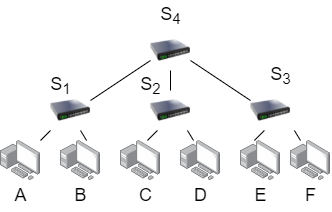
\includegraphics[width=200px]{images/4_Switched_Networks/layered_switch.png}
\end{figure}
Quest strutture sono utili per organizzare le reti in base alla posizione.
Se A vuole inviare un frame ad E invierà il frame inizialmente ad $S_1$, se questo ha la entry nella tabella lo invierà ad $S_4$ altrimenti lo invia su tutte le sue interfacce e così via per ogni switch.

Questo genere di rete permette l' eliminazione delle collisioni e quindi un aumento delle performance.
Inoltre permette di supportare diversi tipi di link in quanto gli switch possono avere diversi tipi di interfacce.
Sono semplici da gestire perché se c'è un link danneggiato si può disconnetterlo direttamente dallo switch e sostituirlo.
Aumenta anche la security perché grazie all' instradamento selettivo si limita di molto lo sniffing dei pacchetti (si può sempre eseguire un poisoning delle tabelle di switching).


\subsection{VLANs}
Riprendiamo la topologia gerarchica precedente, notiamone alcuni problemi:
\begin{itemize}
    \item il traffico di broadcast è globale per tutta la rete, nonostante logicamente siano 3 reti diverse
    \item abbiamo un utilizzo inefficiente degli switch, in genere hanno molte porte ma noi ne usiamo solo alcune perché vogliamo avere una divisione della rete
    \item se un utente di una rete si spostasse di reparto ma volesse continuare ad essere connesso alla stessa sottorete di prima non potrebbe farlo senza tirare nuovi cavi
\end{itemize}
Per risolvere questi ed altri problemi sono state inventate le VLAN - Virtual LAN.

\subsubsection{Port-based VLAN}
Si raggruppano le porte di uno switch (tramite opportune configurazioni) in modo che un singolo switch fisico operi come più switch virtuali.
Con questa implementazione otteniamo:
\begin{itemize}
    \item isolamento del traffico: i frame che arrivano da una VLAN non possono andare nell' altra senza passare per un router (quindi forwarding a livello rete)

    \item appartenenza dinamica: le singole porte dello switch possono cambiare VLAN alla quale sono assegnate tramite opportuna configurazione
\end{itemize}

NB: posso anche segnare l' appartenenza di un host ad una VLAN attraverso il suo indirizzo MAC.

\subsubsection{VLAN tra più switch}
Per permettere a diversi switch di instradare traffico sulle VLAN c'è bisogno di un nuovo protocollo che modifichi i frame aggiungendo le informazioni sulle VLAN.
Possiamo configurare le porte che connettono i due switch come \emph{porte trunk} cioè come porte che parlano il protocollo 802.1Q.

Mettiamo in comparazione il formato dei frame ethernet e 802.1Q:
\begin{figure}[H]
    \centering
    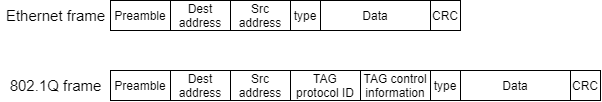
\includegraphics[width=330px]{images/4_Switched_Networks/802.1Q_frame.png}
\end{figure}
i campi in più sono:
\begin{itemize}
    \item Tag protocol identifier: indicano il protocollo usato per le VLAN
    \item Tag control information: contiene l' identificativo della VLAN (12 bit) ed altre informazioni
\end{itemize}
Ovviamente viene ricomputato il CRC su tutto il nuovo frame.

\subsection{Wide-Area Packet-Switched Networks}
Con solamente gli switch possiamo creare delle reti abbastanza grandi in cui l'indirizzamento è basato sull' indirizzo fisico (MAC address) e l' instradamento è effettuato dagli switch attraverso le loro tabelle.

Possiamo creare due tipi di servizi su queste reti:
\begin{itemize}
    \item connectionless: ogni pacchetto è gestito singlarmente, detto anche servizio a datagramma
    \item con connessione: si crea un circuito virtuale prima della trasmissione e tutti i pacchetti poi lo seguono per arrivare a destinazione
\end{itemize}

\subsubsection{ATM - Asynchronous Transfer Mode}
E' uno standard risalente agli anni 90 che aveva come scopo quello di permettere il trasporto di voce, video e dati in maniera efficiente per tutti questi tipi di servizi.

E' un sistema ad instradamento di pacchetti che usa canali virtuali, i pacchetti sono di dimensione fissa e sono chiamati \emph{cells}.

Offre 4 servizi in base al tipo di traffico da instradare:
\begin{itemize}
    \item CBR: constant bit rate
    \item VBR: variable bit rate
    \item ABR: available bit rate
    \item UBR: unspecified bit rate
\end{itemize}

Essendo basato su un circuito virtuale prima di trasmettere i dati si deve effettuare una chiamata in modo da costruire il canale, alla fine invece bisogna distruggerlo, ciò va fatto per ogni flusso di dati che si vuole inviare.

Ogni pacchetto trasporta l' identificativo del canale virtuale, non l' indirizzo del destinatario, ogni switch che incontra nel suo percorso legge questo identificativo e sa verso quale interfaccia instradarlo in quanto conosce il percorso che deve prendere.

Per rendere il servizio predicibile i dispositivi di rete intermedi possono allocare delle risorse al singolo canale virtuale.

Il pacchetto che viene instradato sul canale virtuale oltre a contenere l' identificativo del segnale mantiene anche il numero del link, ogni link nel canale ha un numero univoco che lo identifica e la sequenza di questi numeri è il percorso che costituisce il canale.
Quando uno switch si vede arrivare un pacchetto controlla il numero di link che contiene e l' interfaccia di ingresso, consulta la sua tabella di forwarding e legge l' interfaccia di uscita ed il numero di link di uscita, usa questo numero per sostituire il numero di link che contiene il pacchetto.

Per fare ciò ogni switch deve mantenere in memoria lo stato delle connessioni, quindi è un protocollo stateful.

\subsection{Datagram service}
Non ha bisogno di un setup iniziale, gli switch non devono mantenere informazioni circa lo stato delle connessioni, i singoli pacchetti possono seguire percorsi diversi dalla sorgente alla destinazione in base a metriche opportune per scegliere i link.
I pacchetti vengono indirizzati sulla base del solo indirizzo di destinazione.

\subsection{Virtualizzazione di una rete}
Tutto questo layer si può vedere come una astrazione di una connessione punto-punto.
Il livello superiore chiede di inviare pacchetti verso un certo host destinatario, non gli importa se i due siano connessi direttamente o ci siano altri dispositivi nel mezzo, ciò che vede il layer superiore è una connessione punto-punto.

